%master_report.tex, can't be edited - Mark
% edit the content.tex file instead
\documentclass[a4paper,11pt,hidelinks]{report}
\usepackage[utf8]{inputenc}
\usepackage{amsmath}
\usepackage[titletoc,toc,page]{appendix}

\usepackage[english]{babel}
\usepackage{graphicx}
\usepackage{subcaption}
\usepackage{amssymb}
\usepackage{titlesec}
\usepackage{helvet}
\renewcommand{\familydefault}{\sfdefault}
\usepackage{calc}
\usepackage{amsfonts}
\usepackage{lipsum}
\usepackage[amsmath,amsthm,thmmarks]{ntheorem}
\usepackage{fancyvrb}
\usepackage{setspace}
\usepackage[T1]{fontenc}
\doublespacing
\usepackage{url}
\usepackage{letltxmacro}
%\usepackage{bigints}
\usepackage{soul}
\usepackage[top=20mm,left=20mm,right=20mm,bottom=20mm,footskip=25pt]{geometry} %was 0.14in, don't know why - Mark
\usepackage{fancyhdr}
\usepackage{footnote}
\usepackage{appendix}
\usepackage{siunitx}
\usepackage{multirow}
\usepackage{wrapfig}
\usepackage{textgreek}
\usepackage{longtable}
\usepackage{bigstrut}
\usepackage[table,dvipsnames]{xcolor}
\usepackage{pdfpages}
\usepackage{titling}
\usepackage{csquotes}
\usepackage{pbox}
\usepackage{booktabs}
\usepackage[export]{adjustbox}
\usepackage{array}
\newcolumntype{C}[1]{>{\centering\arraybackslash}p{#1}}
%\usepackage{pbox}
\usepackage{rotating}   % added by Mark for use in table
\usepackage{pifont}     % added by Mark to include tick symbols in table
\usepackage{listings}   % added by Xiaonan to include Matlab code
\lstset{
basicstyle=\small\ttfamily,
columns=flexible,
breaklines=true
}
\usepackage{caption}    % changed to caption / should still work
\usepackage{tocloft}    % added by Mark for TOC names
\usepackage{textcomp}
\setcounter{tocdepth}{4}
\setcounter{secnumdepth}{4}

%References & bibliography - add your own .bib files with \addbibresource command
\usepackage[backend=bibtex,style=numeric-comp,sorting=none]{biblatex}   % Disabled Sorting - Mark
\DeclareBibliographyAlias{webpage}{online}  %ignore warnings
\addbibresource{bibliography.bib}

\AtBeginDocument{\let\latexlabel\label}

\titleformat{\chapter}[hang]
{\normalfont\huge\bfseries}{\thechapter}{17.5pt}{\huge}
\titlespacing*{\chapter}{0pt}{-40pt}{0pt}
\titlespacing*{\section}{0pt}{0pt}{0pt}
\titlespacing*{\subsection}{0pt}{0pt}{0pt}
\titlespacing*{\subsubsection}{0pt}{0pt}{0pt}   %reduce spacing to fit with other stuff

%Remove the Page number from the part pages - Mark
\makeatletter
\renewcommand\part{%
    \if@openright
    \cleardoublepage
    \else
    \clearpage
    \fi
    \thispagestyle{empty}%   % Original »plain« replaced by »emptyx
    \addtocounter{page}{-1} %Decrease the page counter so the part page doesn't count, added by Mark
    \if@twocolumn
    \onecolumn
    \@tempswatrue
    \else
    \@tempswafalse
    \fi
    \null\vfil
    \secdef\@part\@spart}
\makeatother
% From http://tex.stackexchange.com/questions/54115/how-to-let-part-stay-solo-page-and-no-page-number


\newcommand\numberthis{\addtocounter{equation}{1}\tag{\theequation}}
% All sqrts closed
\LetLtxMacro{\oldsqrt}{\sqrt}
\renewcommand{\sqrt}[1][]{%
    \def\DHLindex{#1}\mathpalette\DHLhksqrt}
\def\DHLhksqrt#1#2{%
    \setbox0=\hbox{$#1\oldsqrt[\DHLindex]{#2\,}$}\dimen0=\ht0
    \advance\dimen0-0.2\ht0
    \setbox2=\hbox{\vrule height\ht0 depth -\dimen0}%
    {\box0\lower0.71pt\box2}}

\makeatletter
\newcommand*\@dblLabelI {}
\newcommand*\@dblLabelII {}
\newcommand*\@dblequationAux {}

\def\@dblequationAux #1,#2,%
{\def\@dblLabelI{\label{#1}}\def\@dblLabelII{\label{#2}}}

\newcommand*{\doubleequation}[3][]{%
    \par\vskip\abovedisplayskip\noindent
    \if\relax\detokenize{#1}\relax
    \let\@dblLabelI\@empty
    \let\@dblLabelII\@empty
    \else % we assume here that the optional argument
    % has the required shape A,B
    \@dblequationAux #1,%
    \fi
    \makebox[0.5\linewidth-1.5em]{%
        \hspace{\stretch2}%
        \makebox[0pt]{$\displaystyle #2$}%
        \hspace{\stretch1}%
    }%
    \makebox[0.5\linewidth-1.5em]{%
        \hspace{\stretch1}%
        \makebox[0pt]{$\displaystyle #3$}%
        \hspace{\stretch2}%
    }%
    \makebox[3em][r]{(%
        \refstepcounter{equation}\theequation\@dblLabelI,
        \refstepcounter{equation}\theequation\@dblLabelII)}%
    \par\vskip\belowdisplayskip
}
\makeatother
\renewcommand{\headrulewidth}{0pt}

% For multi-line cells - see http://tex.stackexchange.com/questions/2441/how-to-add-a-forced-line-break-inside-a-table-cell
\newcommand{\multicell}[2][c]{%
    \begin{tabular}[#1]{@{}c@{}}#2\end{tabular}}

\setlength{\headheight}{13.6pt}


%Toc indents and dimensions
\setlength{\cftsecindent}{1.5em}
\setlength{\cftsecnumwidth}{2.8em}

\setlength{\cftsubsecindent}{4.0em}
\setlength{\cftsubsecnumwidth}{3.6em}

\setlength{\cftsubsubsecindent}{7.4em}
\setlength{\cftsubsubsecnumwidth}{4.5em}

\usepackage{hyperref}

\pretitle{%
    \begin{center}
        %\LARGE
        
\includegraphics[width=4.5cm]{Images/cover.jpg}\\ \Huge%[\bigskipamount]
    }
    \posttitle{\end{center}}

% Title Page
\title{Analysis of Activity Data from Smartphones}
\author{Jamieson Brynes, Somerville College}


%Table of contents command by Mark
% use \setauthor{<name>} just before the chapter/section/subsection heading you want to assign to <name>
%for example:
%\setauthor{Mark}
%\chapter{Optical Tweezing}
%
%Also, you can put whatever you want to appear on the left in the toc in square brackets.
%for example:
%\chapter[OT]{Optical Tweezing} will be printed as OT in the table of contents

\makeatletter
\renewcommand{\@pnumwidth}{2.3em}
\newcommand{\setauthor}[1]{%
    \addtocontents{toc}{\protect\@namedef{authortag}{#1}}%
}

\newcommand{\putafterpnum}{%
    \ifcsname authortag\endcsname
    \makebox[0pt][r]{\smash{\colorbox{white}{\strut\authortag}\hspace{\@pnumwidth}}}%
    \global\let\authortag\relax
    \fi
}

\renewcommand{\cftchapafterpnum}{\putafterpnum}
\renewcommand{\cftsecafterpnum}{\putafterpnum}
\renewcommand{\cftsubsecafterpnum}{\putafterpnum}
\renewcommand{\cftsubsubsecafterpnum}{\putafterpnum}

\makeatother

\begin{document}

\maketitle
\pagestyle{fancy}

\pagenumbering{gobble}
\section*{\centering{Acknowledgements}}

    In addition to the guidance and advice offered to me by my supervisor Lionel Tarassenko, I would also like to acknowledge the contributions of Carmelo Velardo and Dario Salvi to this project. They gave me their time and advice as well as agreeing to walk around the Institute of Biomedical Engineering with pink straps on their legs and feet to aid me in data collection. These three outstanding individuals were more than generous and their contributions were invaluable to the success of this project.

\begin{abstract}

    Chronic diseases affect large sections of the general population and incur large costs to the healthcare system, to the tune of \$1.4 trillion per year in the United States. Patients with chronic diseases require regular evaluation through the collection and analysis of data. This project set out to evaluate the information that could be extracted from accelerometer data for people living with chronic diseases. Algorithms were developed for step counting using the accelerometer within a smartphone device and for sleep detection using a wrist-mounted accelerometer. These algorithms derived two metrics of interest to healthcare professionals, the level of activity and sleep quality. Since smartphones and wearables have high penetration in the population and continue to proliferate, healthcare professionals would be able to utilize these algorithms to enable remote data collection. 

    The step-counting algorithm is modular and based on the Windowed Peak Detection design. A ground-truth device was designed to enable rapid data collection for optimization and validation of the step-counting algorithm. A database was created from the data recordings acquired using this ground-truth device. The database was used to optimize the step counting algorithm resulting in a median step counting accuracy of 96.8\% across the entire database. Optimization for specific scenarios was also performed giving high accuracy, up to 99\% in some cases. 

    The sleep-detection algorithm is based on classification with logistic regression. A publicly available database was utilized for the optimization of this algorithm. A filter with a hard-limiter after was used to process the logistic regression output giving results that more closely resemble sleep patterns. This methodology gives a median total time asleep error of 10.9\%. This improves upon previous attempts on the same database by approximately 10\%. 

    The source code for both algorithms will be released along with the step-counting database that was created during the project. The high accuracy achieved by the step counting algorithm means that it is ready to be implemented in a medical context, for example, in the six minute walk test which is a standard procedure for evaluating the capabilities of patients with congestive heart failure. The improvements achieved by the sleep detection algorithm are a step forward and the nature of the algorithm allows for further refinements and improvements.
\end{abstract}
\pagenumbering{roman}
\tableofcontents
\newpage
\pagenumbering{arabic}
\setcounter{page}{1}


\part{Introduction}

    \chapter{Motivation}

        \section{Pulmonary Disease and Heart Failure}

        \section{Six Minute Walk Test}

    \chapter{Objectives}

        \section{Step Counter}

        \section{Sleep Detection}

    \chapter{Literature Review}
\part{Step Counter Algorithm}

    \chapter{Overview}

        This section covers the development and evaluation of the step counter algorithm. The algorithm aims to extract incidences of steps from the raw accelerometer data recorded on a smartphone. An example of raw accelerometer data of walking is shown below in Figure \ref{img_accel_ex}. It should be quite clear that the act of walking gives rise to periodic activity with a period corresponding to a single step. The act of walking is detailed in Naqvi, et. al. [CIT] and is as follows:

        \begin{enumerate}
            \item At the beginning of the step, the planted foot is pushed backwards into the floor.
            \item Static friction opposes this force. This provides the driving force forward.
            \item At the end of the step the stepping foot is placed on the floor and pushes forward into the floor.
            \item Again, static friction opposes this force, giving rise to a backwards force.
        \end{enumerate}

        \begin{figure}[h]
            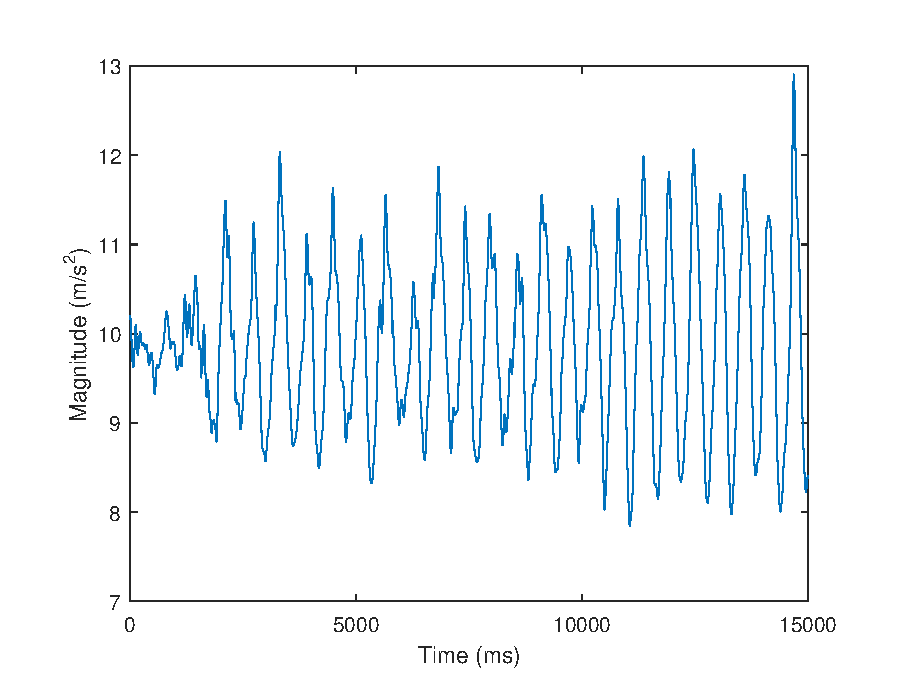
\includegraphics[width=\textwidth]{Images/accel_signal.eps}
            \centering
            \caption{Example of an accelerometer signal recorded during a period of walking.}
            \label{img_accel_ex}
        \end{figure}

        It is clear that each step will have both a peak and a trough associated with 2 and 4 respectively. The algorithm shall identify the peaks in the accelerometer signal. Effectively, the problem is one of peak detection in a noisy signal. 

        The algorithm is split into five stages, each responsible for a particular function. The data flows from stage to stage. All stages have an input data stream and output data stream, with the exception of the final stage which only has an input data stream. A block diagram is shown below in Figure \ref{img_sc_block}. Each one of the five stages will be described in detail in the following section.

        \begin{figure}[h]
            \includegraphics[width=\textwidth]{Images/step_counter_block.png}
            \centering
            \caption{Block diagram of the step counter algorithm.}
            \label{img_sc_block}
        \end{figure}

    \chapter{Algorithm Description}

        \section{Pre-Processing Stage}

            The Pre-Processing Stage is responsible for two functions:

            \begin{enumerate}
                \item Formatting the data received from the accelerometer into a usable format.
                \item Ensuring a constant sampling frequency by means of linear interpolation.
            \end{enumerate}

            The accelerometer data is received in the tri-axial format, however the algorithm is concerned with the magnitude rather than any single directional component because the the physical orientation of the device is unknown. The time stamps of the samples should also be scaled appropriately so that the first sample received from the user initiating the algorithm is at $t = 0$. The time stamps of the samples are provided in nanoseconds and are not given in standard UTC format, but as the time since system boot. The equations for these operations are simple and are as follows:

            \begin{equation}
                m = \sqrt{a_{x}^2 + a_{y}^2 + a_{z}^2},
            \end{equation}

            \begin{equation}
                t_{i,adjusted} = \frac{t_i - t_0}{t_s},
            \end{equation}

            where $m$ is the magnitude of the acceleration signal, $a_{x}$ is the acceleration in the x direction, $a_{y}$ is the acceleration in the y direction, $a_{z}$ is the acceleration in the z direction, $t_{i,adjusted}$ is the adjusted time stamp for the i-th sample, $t_i$ is the time stamp for the i-th sample, $t_0$ is the first time stamp in the trace, and $t_s$ is the time-scaling factor. For example, converting from nanoseconds to milliseconds, $t_s = 10^6$. 

            The data is then inserted into a simple data structure and is appended to an internal buffer of size 2. When this buffer is full, we will interpolate between these two points. The reason interpolation is needed is that although the developer can specific a desired sample rate in the Android application, there is no guarantee that the accelerometer will be sampled at this rate. An example of this is shown below in Figure \ref{img_sampling_freq} where time between samples is plotted against samples. For the filtering stage, we need to ensure that the data is sampled at a constant rate.

            The algorithm knows what the desired sample rate is, and will interpolate at this value. For example, if the sample rate is set to $f = 100 Hz$, then the algorithm will interpolate around $t = 0, 10, 20, 30, ... ms$. Each interpolated point is appended to the end of the stage's output data stream. The pseudocode for the linear interpolation is shown below.

            The equation for linear interpolation is as follows:

            \begin{equation}
                value = \frac{y_1 - y_0}{t_1 - t_0} t_{int} + y_0,
            \end{equation}

            where the two points that are being interpolated between are given by: $(t_1, y_1)$ and $(t_0, y_0)$, and the time to be interpolated at is given by $t_{int}$.

            \begin{figure}[h]
                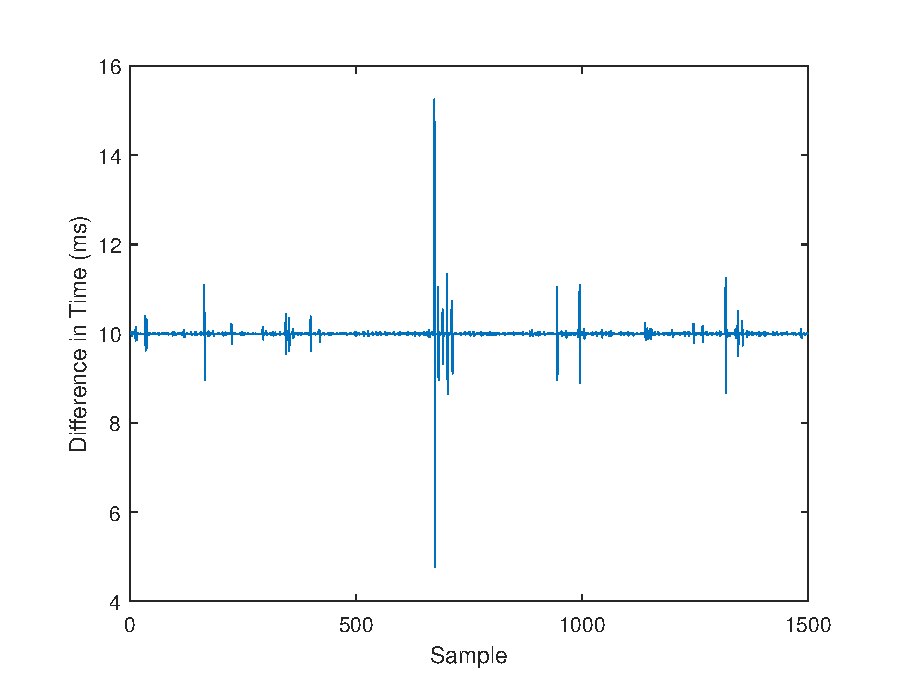
\includegraphics[width=\textwidth]{Images/sampling_freq.eps}
                \centering
                \caption{Time differences between samples for a 100Hz sampled signal. Note that the non-constant sampling times leads to the requirement for interpolation.}
                \label{img_sampling_freq}
            \end{figure}

        \section{Filtering Stage}

            The function of the filtering stage is to smooth the signal by removing as much of the high frequency noise from the acceleromater as possible.

            The filter required is a simple finite impulse response (FIR), low-pass digital filter. Ideally, this would be a steep-low pass filter with a frequency response described by Figure \ref{img_ideal_filter} below. However, this is impossible to achieve due to the infinite impulse response in the time domain (top-hat transforms to the sinc function). In order to capture the a variety of walking speeds, the cutoff of these filters will aim to be around 3 Hz. This should be sufficient to capture the walking of even the speediest walkers, as this would translate to an pace of $5.4 mph$ according to the ratio of $2000 steps = 1 mile$ as given by the American College of Sports Medicine [CIT]. Note that the average walking pace was found to be $3.1 mph$ in a study by Knoblauch, et. al. [CIT].

            An example of the prefiltered signal and the filtered signal is shown below in Figure \ref{img_filtered_signal}.

            \begin{figure}[h]
                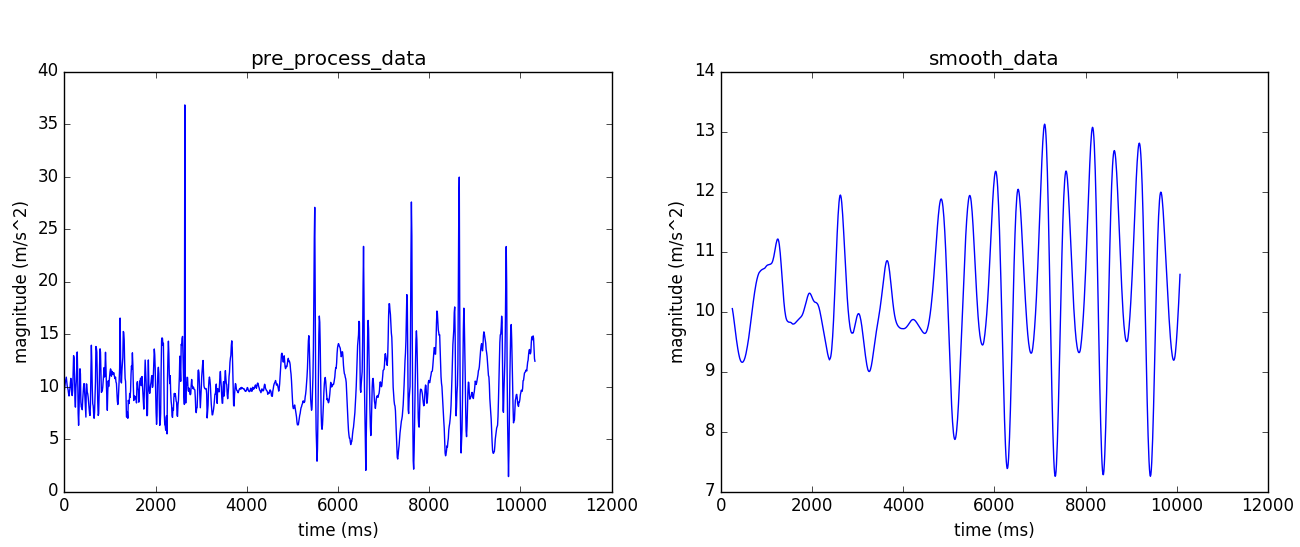
\includegraphics[width=\textwidth]{Images/filtered_signal.png}
                \centering
                \caption{Example of a signal being filtered. Filter used: Gaussian Filter with $N=51$ and $\sigma=0.35$. Note the large peaks due to noise are filtered out entirely.}
                \label{img_filtered_signal}
            \end{figure}

            A few filters were implemented for performance testing.

            \subsection{Moving Average}

                This is a very simple filter, each point in the filter window are weighted equally such that:

                \begin{equation}
                    m_k = \frac{1}{N},
                \end{equation}

                where $m_k$ is the $k^{th}$ filter coefficient, and $N$ is the length of the filter. The frequency response of this filter is shown below in Figure \ref{img_cm_filter}.

                \begin{figure}[!th]
                    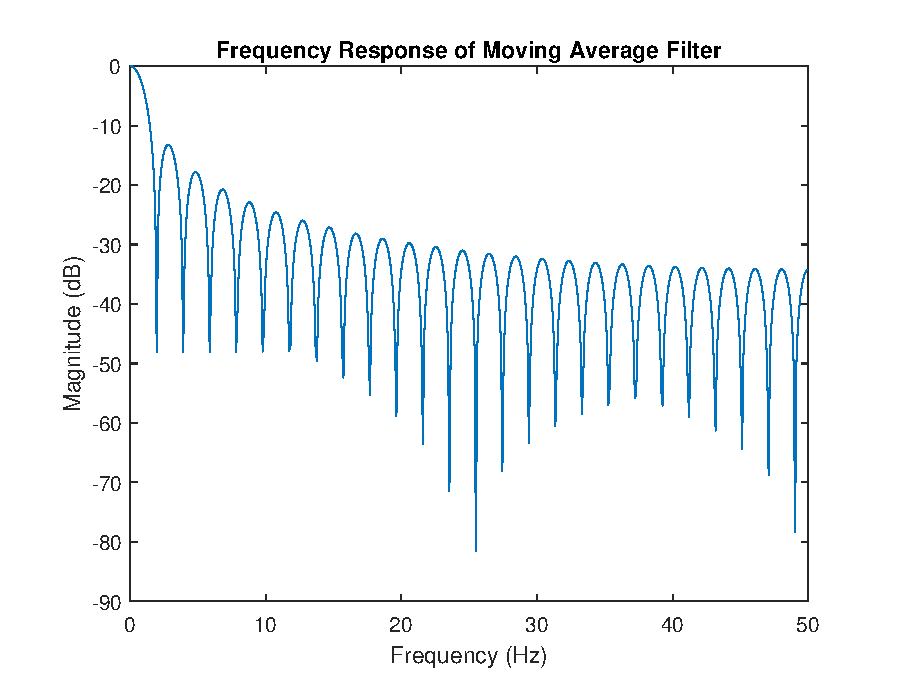
\includegraphics[width=\textwidth]{Images/cm_filter.eps}
                    \centering
                    \caption{Frequency response of the moving average filter with $N=31$.}
                    \label{img_cm_filter}
                \end{figure}

            \subsection{Gaussian Filter}

                This is a more complex filter, using a Gaussian as the waveform for the filter coefficients. This filter attempts to suppress the sidelobes of the center moving average filter by having a smoother transition to 0 magnitude. The weights of the filter are given by:

                \begin{equation}
                    g_k = \exp(-\frac{1}{2}(\frac{k - \frac{N-1}{2}}{\sigma \frac{N-1}{2}})^2),
                \end{equation}

                where $g_k$ is the $k^{th}$ coefficient of the filter, $N$ is the length of the filter window, and $\sigma$ is a parameter defining the standard deviation of the Gaussian. Note that the standard deviation also scales with the length of the filter. The frequency response of this filter is shown below in Figure \ref{img_ga_filter}.

                \begin{figure}[!th]
                    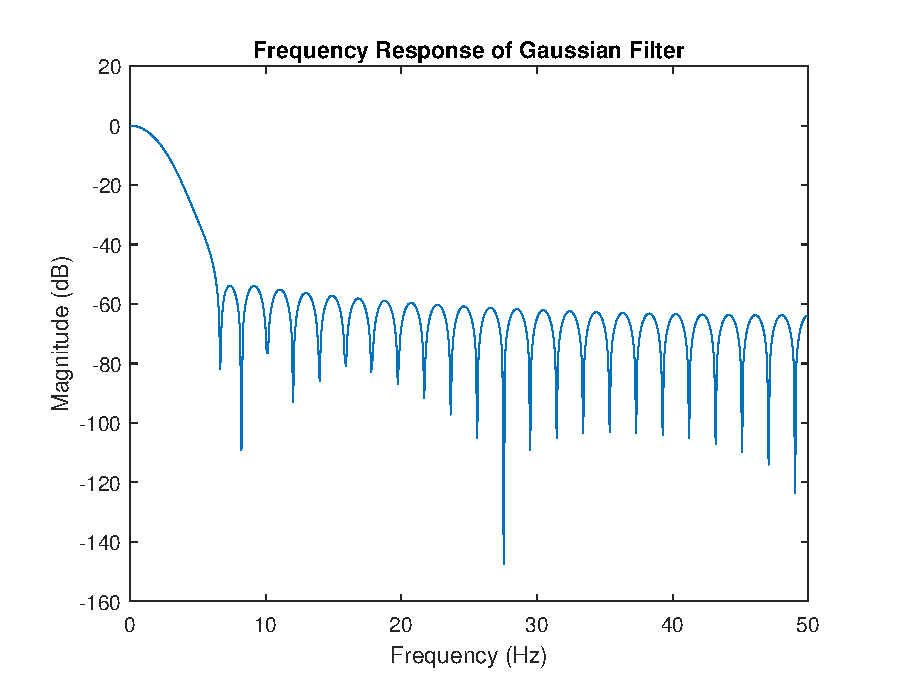
\includegraphics[width=\textwidth]{Images/ga_filter.eps}
                    \centering
                    \caption{Frequency response of the Gaussian filter with $N=51$ and $\sigma = 0.35$.}
                    \label{img_ga_filter}
                \end{figure}

            \subsection{Hann Filter}

                This is a similar filter to that of the Gaussian, where it attempts to smooth out the response by suppressing the sidelobes of the center moving average filter. The weights of the filter are derived from the Hann window [CIT] and are as follows: 

                \begin{equation}
                    h_k = \frac{1}{2}(1 - \cos(\frac{2\pi k}{N - 1}))
                \end{equation}

                where $h_k$ is the $k^{th}$ filter coefficient and $N$ is the length of the filter window. The frequency response of this filter is shown below in Figure \ref{img_ha_filter}.

                \begin{figure}[!th]
                    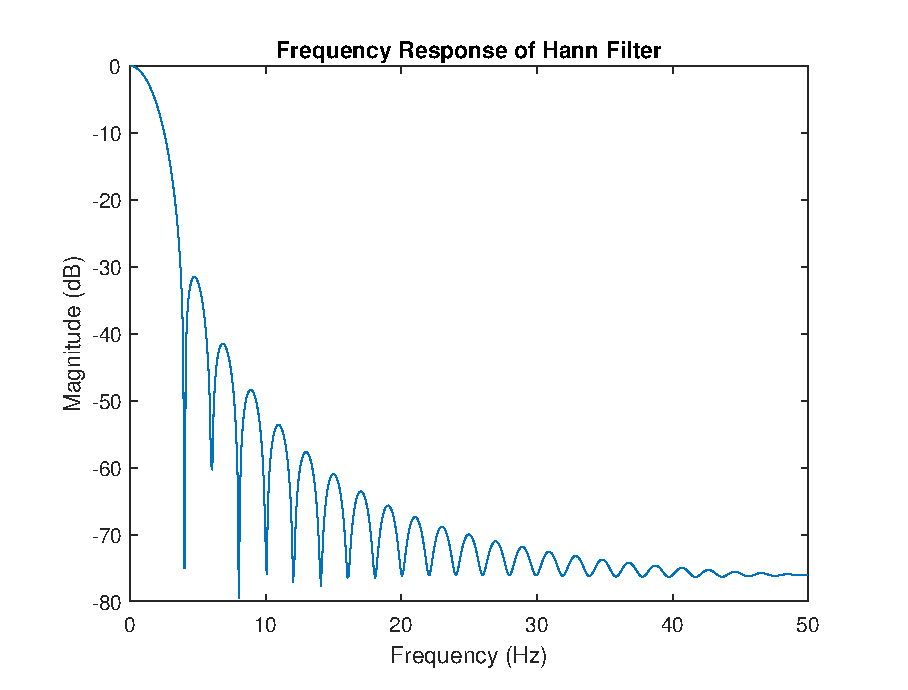
\includegraphics[width=\textwidth]{Images/ha_filter.eps}
                    \centering
                    \caption{Frequency response of the Hann filter with $N=51$.}
                    \label{img_ha_filter}
                \end{figure}  

            \subsection{Kaiser-Bessel Filter}

                This is the most complex filter design, designed by Kaiser [CIT] in order to achieve the desired attenutation at the cutoff frequency. It combines the ideal filter response (note a sinc function in the time domain) and a Bessel window to achieve the result. The calculation of the coeffcients are as follows.

                First, calculate the window shape parameter $\alpha$. 

                \begin{equation}
                    \alpha = 
                        \begin{cases}
                            0.1102(A - 8.7) & A \ge 50 \\
                            0.5842(A-21)^{0.4} + 0.07886(A-21) & 21 \leq A \geq 50 \\
                            0 & A \le 21
                        \end{cases},
                \end{equation}

                where $A$ is the desired attenuation at the cutoff frequency.

                Then calculate the coefficients of the Kaiser-Bessel window:

                \begin{equation}
                w_k = \frac{I_0(\alpha \sqrt{1 - (\frac{k - N_p}{N_p})^2})}{I_0(\alpha)},
                \end{equation}

                where $w_k$ is the $k^{th}$ coefficient of the window, $\alpha$ is the window shape parameter, $N_p$ is the midpoint of the filter, $N_p = \frac{N-1}{2}$ where $N$ is the length of the filter, and $I_0$ is the $0^{th}$ order Bessel function of the first kind.

                Then calculate the coefficients of the ideal filter response:

                \begin{equation}
                i_k = \frac{\sin(2\pi k\frac{F_c}{F_s})}{\pi k},
                \end{equation}

                where $i_k$ is the $k^{th}$ coefficient of the ideal filter response, $F_c$ is the desired cutoff frequency and $F_s$ is the sampling frequency.

                Finally, compute the coefficients of the filter with: 

                \begin{equation}
                b_k = w_ki_k,
                \end{equation}

                where $b_k$ is the $k^{th}$ coefficient of the Kaiser-Bessel filter response. The frequency response of this filter is shown below in Figure \ref{img_kb_filter}.

                \begin{figure}[!th]
                    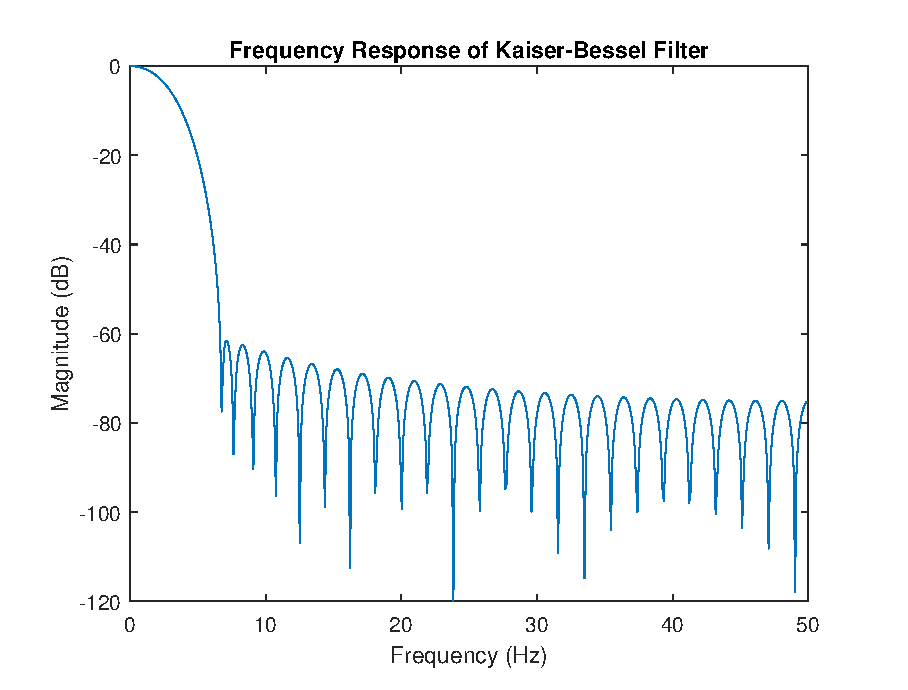
\includegraphics[width=\textwidth]{Images/kb_filter.eps}
                    \centering
                    \caption{Frequency response of the Kaiser-Bessel filter with $N=51$, $A=60dB$, $F_c = 3Hz$, and $F_s= 100Hz$.}
                    \label{img_kb_filter}
                \end{figure}  

        \section{Scoring Stage}

            The function of the scoring stage is to evaluate how 'peaky' any given point is. The result of this stage should increase the the magnitude of peak points, making them more obvious to a peak detector.

            A few methods were developed to be used in testing. These are detailed below.

            \subsection{Maximum Difference}

                This method uses the local neighbors of the point in question to determine how peaky the point is. It will look $N$ points to the left and determines the maximum difference between the point in question and those points. It will do the same for the $N$ points to the right, and then average the two maximum differences as the result.

                This operation will result in exaggerating peaks corresponding to steps as the following trough will cause a higher magnitude relative to peaks corresponding to other causes. An example of the output from a filtered signal to the scored signal using Maximum Difference is shown below in Figure \ref{max_diff_score}.

                The equation describing this behavior is given by:

                \begin{equation}
                x = \frac{\max\limits_k{(x_i - x_{i-k})} + \max\limits_k{(x_i - x_{i+k})}}{2},
                \end{equation}

                where $i$ is the point under consideration, and $x_n$ is the value of the signal at the $n^{th}$ sample.

                \begin{figure}[!th]
                    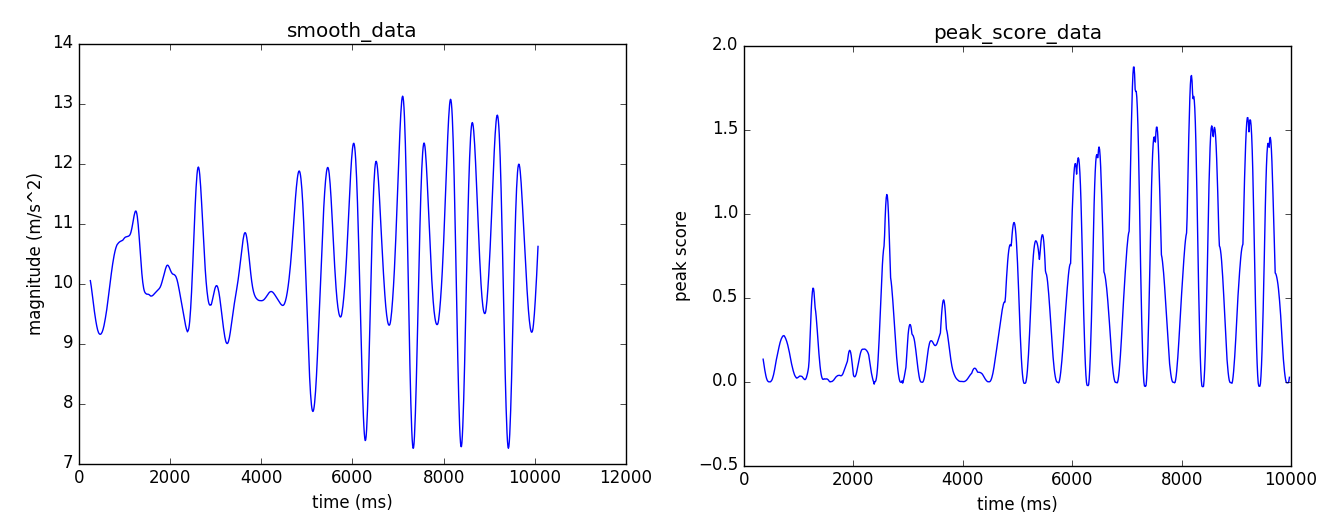
\includegraphics[width=\textwidth]{Images/max_diff_score.png}
                    \centering
                    \caption{Peak Scoring using Maximum Difference with $N=6$. Filtered data is on the left, smoothed data is on the right. Note how the large peaks are amplified, while the smaller ones are suppressed.}
                    \label{max_diff_score}
                \end{figure}                 

            \subsection{Mean Difference}

                This method is similar to Maximum Difference, except that instead of taking the maximum of the difference to the left and the right, Mean Difference takes the mean of all the differences. The effect is similar to Maximum Difference, but smaller in magnitude. It also preserves the overall shape of the waveform.

                An example of the output from a filtered signal to the scored signal using Mean Difference is shown below in Figure \ref{mean_diff_score}.

                The equation describing this behavior is given by:

                \begin{equation}
                x = \frac{\sum_{k=-N, k\neq i}^{N} (x_i - x_{i+k})}{2N},
                \end{equation}

                where $i$ is the point under consideration, $x_n$ is the value of the signal at the $n^{th}$ sample, and $N$ is the characteristic length of the Mean Difference operation.

                \begin{figure}[!th]
                    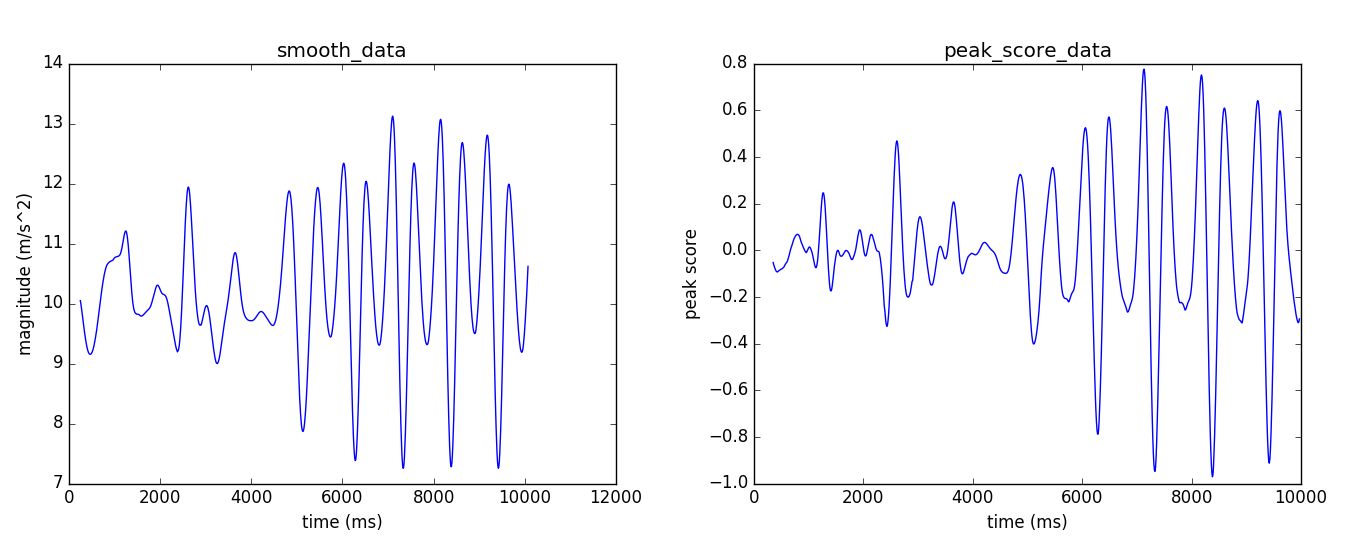
\includegraphics[width=\textwidth]{Images/mean_diff_score.png}
                    \centering
                    \caption{Peak Scoring using Mean Difference with $N=10$. Filtered data is on the left, scored data is on the right.}
                    \label{mean_diff_score}
                \end{figure}

            \subsection{Modified Pan-Tompkins Scoring}

                This method is a derivative from the famous algorithm by Pan and Tompkins [CIT] that was used for peak detection. 

                The original algorithm had four main steps: digital bandpass filter, differentiate the signal, square the signal, then a moving integration window to reconstitute the signal.

                From this baseline, a modified algorithm was developed:

                \begin{itemize}
                    \item Locally zero-mean the data around with a window of size $N$.
                    \item Set all the data points that are less than 0 to zero.
                    \item Square the data to amplify any large peaks.
                \end{itemize}

                The first step is integral as it ensures that when the data is squared, only truly large peaks get amplified. The second step is important to ensure that only positive peaks get detected. Without this, the algorithm would detect both the peak and trough.

                An example of this scoring using this method is shown below in Figure \ref{pan_tompkins_score}.

                \begin{figure}[!th]
                    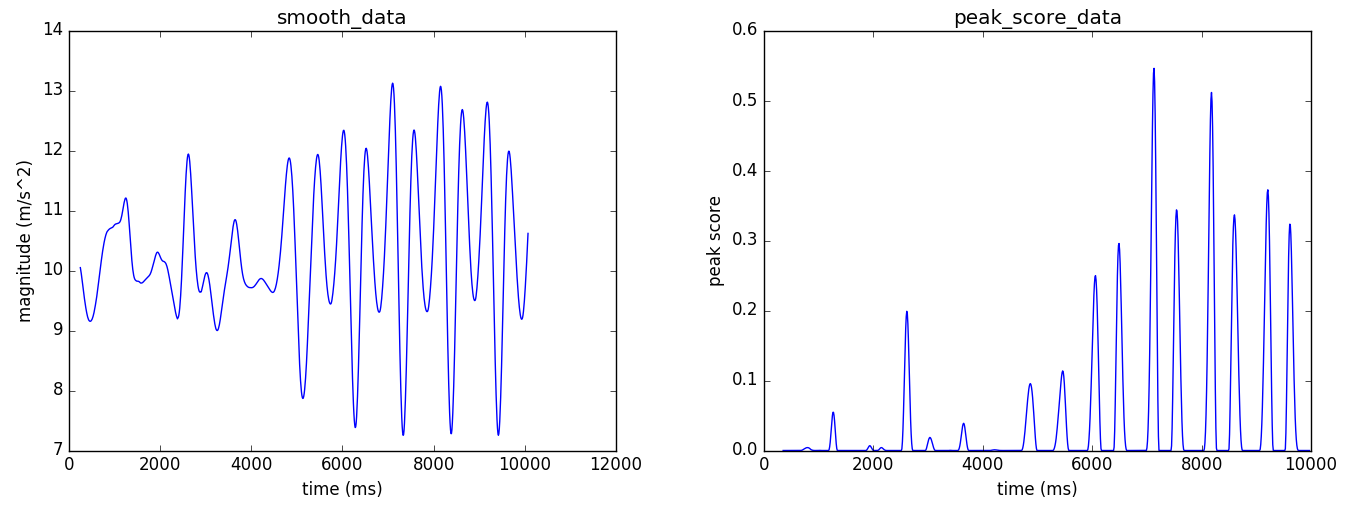
\includegraphics[width=\textwidth]{Images/pan_tompkins_score.png}
                    \centering
                    \caption{Peak Scoring using Modified Pan-Tompkins with $N=10$. Filtered data is on the left, scored data is on the right.}
                    \label{pan_tompkins_score}
                \end{figure}


        \section{Detection Stage}

            The next stage in the process is to identify potential candidates for peaks associated with peaks. This is done using statistics to identify outliers. 

            As the algorithm traverses the signal, it keeps track of a running mean and standard deviation. Computationally efficient way of doing this incrementally are as shown below:

            \begin{equation}
                \bar{x}_n = \frac{x_n + (n-1)\bar{x}_{n-1}}{n},
            \end{equation}

            \begin{equation}
                \sigma_n^2 = \frac
                {(n-2)\sigma_{n-1}^2 + (n-1)(\bar{x}_{n-1} -\bar{x}_n)^2 + (x - \bar{x}_n)^2}
                {n-1},
            \end{equation}

            where $x_n$ is the $n^{th}$ sample, $\bar{x}_n$ is the running mean at the $n^{th}$ sample, and $\sigma_n$ is the running standard deviation at the $n^{th}$ sample.

            The algorithm will then use these two quantities to determine whether any given point is an outlier by thresholding. That is to say, if a point is $c$ or more running standard deviations above the running mean, then it is marked as a potential peak.

            \begin{equation}
                \frac{x_n - \bar{x}_n}{\sigma_n} \stackrel{?}{\geq} c,
            \end{equation}

            where $c$ is the designated threshold.

            An example of the results of this method is shown below in Figure \ref{img_detection_stage}.

            Note that the algorithm skips a number of points at the beginning as it builds up a running mean and standard deviation. Unfortuntely, this means that, almost always, the first peak it encounters will be marked as a potential step.

            \begin{figure}[!th]
                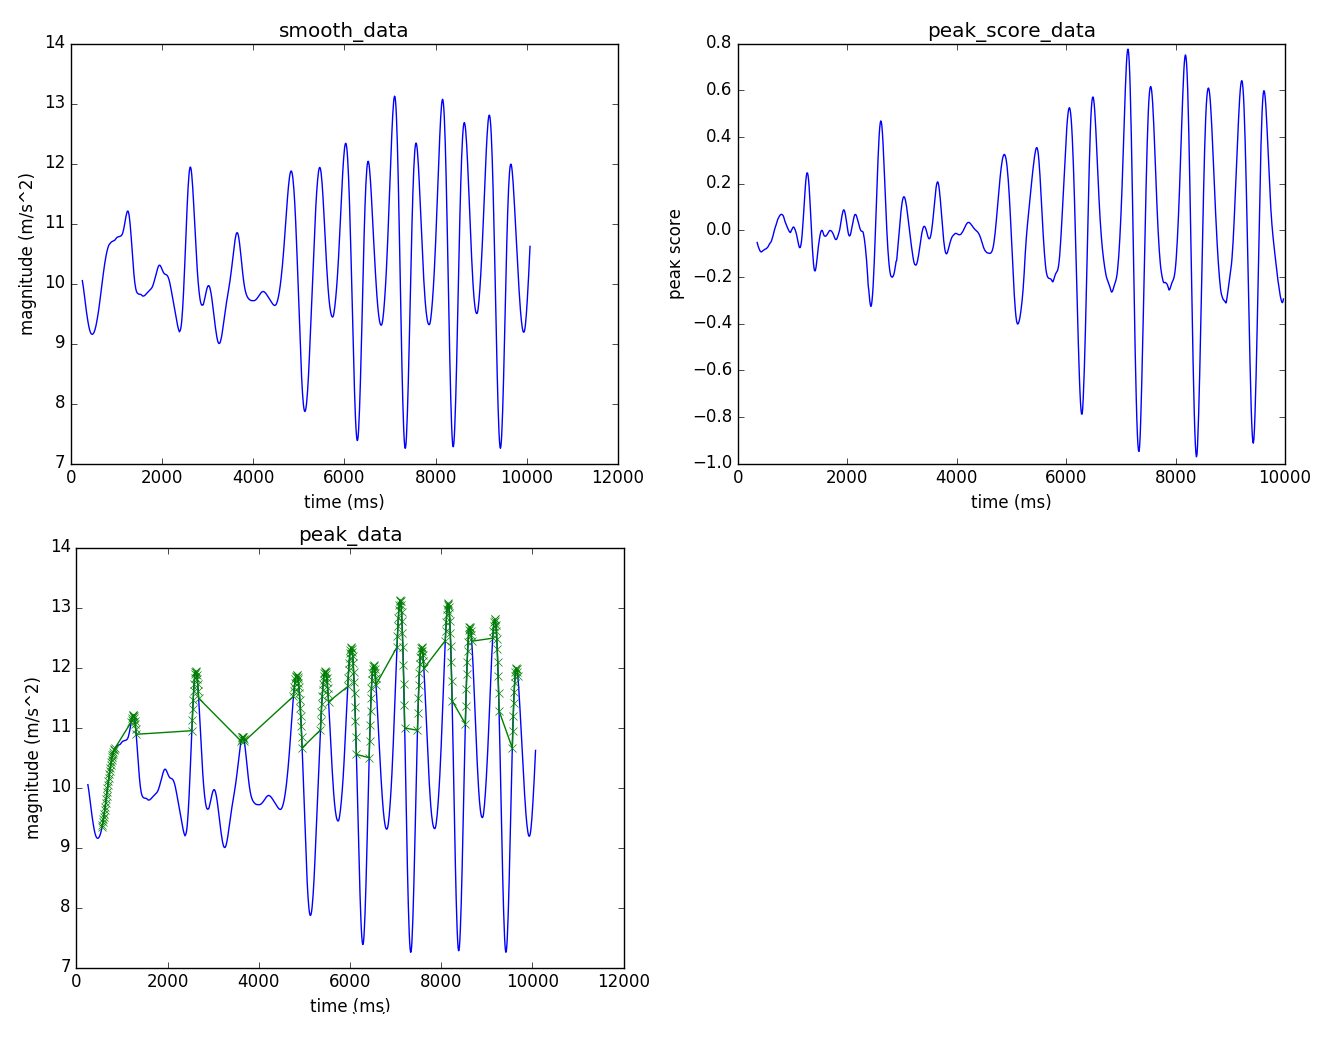
\includegraphics[width=\textwidth]{Images/detection_stage.png}
                \centering
                \caption{The results of the Peak Detection stage. Top Left: filtered signal, Top-Right: scored signal, Bottom-Left: filtered signal with potential peaks overlaid in green. $c=1.2$ for the Peak Detection stage.}
                \label{img_detection_stage}
            \end{figure}


        \section{Post-Processing Stage}

    \chapter{Data Collection Apparatus}

    \chapter{Algorithm Optimization}

    \chapter{Results}

    \chapter{Further Work}

\end{document}